\documentclass[11pt]{article}
\usepackage[utf8]{inputenc}
\usepackage{graphicx}
\graphicspath{ {res/} }
\usepackage{svg}
\usepackage{hyperref}
\usepackage[a4paper,width=150mm,top=25mm,bottom=25mm]{geometry}

\title{
\centering
\begin{minipage}{4cm}
    \centering
    \includesvg[width=4cm]{res/ai-center.svg}
\end{minipage}
\hfill % Add horizontal space
\begin{minipage}{4cm}
    \centering
    \includesvg[width=4cm]{res/un.svg}
\end{minipage}\\[1cm] % Add vertical space
{\large Practical Work - Project Report}\\
\textbf{SemUN: A Semantics-Powered Search Platform for the United Nations' Digital Library}
}




\author{
    Clément Sicard\\
    \texttt{csicard@ethz.ch}\\
    D-INFK, ETH Zurich\\
    \\ 
    \textit{Supervised by:}\\
    Dr. Menna El-Assady$^1$, Dr. Sascha Langenbach$^1$, Catherine Pysden, MSc.$^2$\\
    \\
    $^1$ETH Zurich $^2$United Nations
}

\begin{document}

\maketitle

\begin{center}
	\small\textbf{Keywords}:\\
        \textit{
            Natural Language Processing (NLP), 
            Named Entity Recognition (NER), 
            Graph databases,
            Frontend,
            Network Visualization
        }
\end{center}

\section{Introduction} \label{intro}
The \href{https://digitallibrary.un.org/}{United Nations Digital Library (UNDL)} is a United Nations (UN) service that provides public access to a diverse range of UN documents: voting data, speeches, maps, and open access publications starting from 1979.
All of these documents have been classified according to the \href{https://metadata.un.org/thesaurus/about?lang=en}{UNBIS Thesaurus}, a multilingual database of the controlled vocabulary used to describe UN documents and other materials in the Library's collection, with a more or less precise topic label.

The main idea of this project is to create an analysis platform, with a network visualization of documents from a subset of the documents in the UN Digital Library. The analytics platform will include a basic Named Entity Recognition (NER) system to extract mentioned entities from the documents. The visualization part will be a network visualization, leveraging the versatility of the structure of a graph to display the extracted insights. Both parts aim at improving the search of documents by implementing an analytics layer on top of the existing search engine from the digital library. Various use cases are conceivable. For instance, the tool could be used to get a quick overview of documents in which speaker $X$ has commented on topic $Y$ in year $Z$ --- a functionality of interest to UN staff and member-state delegates alike. Similarly, the tool could be used to discover new documents through shared topics or authorship. 

The submission will include a machine-learning pipeline alongside both a backend and a frontend, with a focus on producing clean and maintainable code.

\section{Administrative details} \label{admin}

This project will be conducted within the framework of the \href{https://ethz.ch/content/dam/ethz/special-interest/infk/department/Images%20and%20Content/Studies/Forms%20and%20Documents/Memo_Practical%20Work.pdf}{practical work}, which is a mandatory part the MSc in Computer Science at ETH Zurich.
The submission date is currently set as 6 August 2023, but can be changed after consultation with the supervisors, provided they think the required work is done.

\section{Project scope}

In the short-term, the goal of this project is to provide a MVP of a potential future UN product, in close contact with UN staff to make it conform to their needs. Specifically, this project will focus – as a first iteration – on Catherine Pysden's suggestion, "Women in Peacekeeping".

The project's long-term scope is to be used as a search engine for UN staff, member-state delegates, and members of the general public with an interest in UN topics. Potential future work could include extending the project to the whole UN Digital Library. It could, for instance, also suggest Thesaurus-compliant metadata for untagged documents to facilitate the work of Library staff.


\section{Project description} \label{desc}


The right of Figure \ref{fig:my_label} shows a simplified schema of the current UN Digital Library infrastructure. 

\subsection{Contribution overview}

\begin{figure}[h]
	\centering
	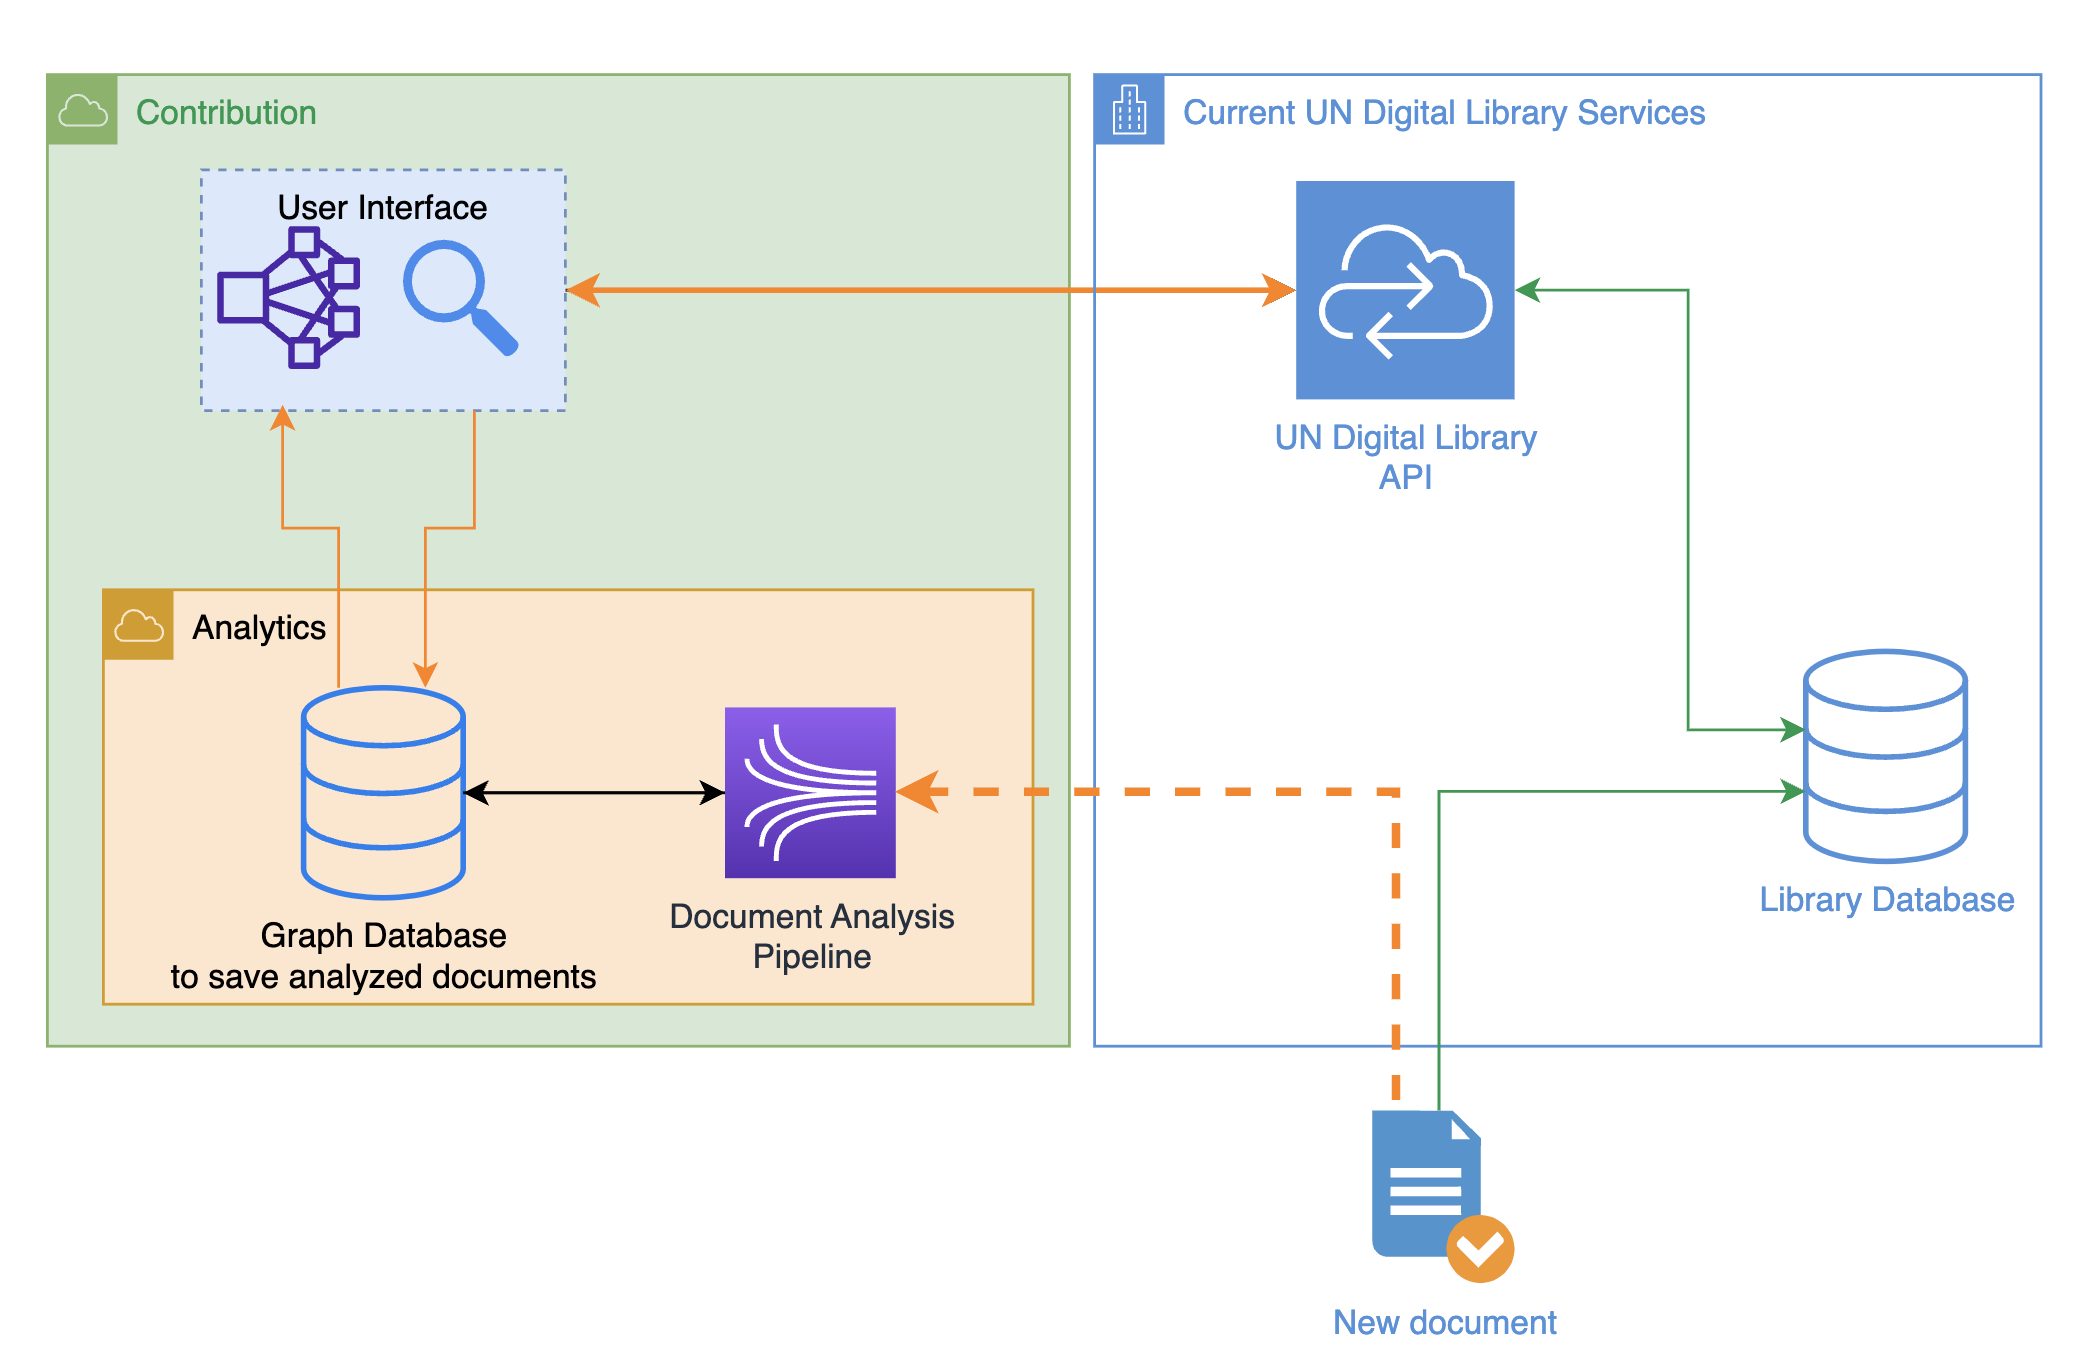
\includegraphics[width=0.9\linewidth]{res/un-infra.png}
	\caption{Proposed architecture, with my contribution in green}
	\label{fig:my_label}
\end{figure}

\subsection{Machine learning pipeline} \label{ml}

The pipeline will be composed of two parts:

\begin{enumerate}
    \item Semantics extraction and summarization
    \item Named entity recognition
\end{enumerate}


\subsubsection{Semantics extraction and summarization}
    
Implementation of semantic analysis techniques to extract meaningful information and insights from the documents. We can think of creating an embedding for each document and generating a summary of its key points. Note that this is likely to be updated depending on UN staff requirements, but that seems to be a safe baseline to start with. It will probably be a transformer-based model from the Hugging Face \href{https://huggingface.co/docs/transformers/index}{\texttt{transformers}} library
    
\subsubsection{Named entity recognition}
Developing/adapting a named entity recognition (NER) model to identify and classify named entities such as organizations, locations, and people mentioned in the documents. For the scope of this project, a reasonable goal is to fine-tune an existing generic NER model on UN acronyms (see \footnote{\href{https://unterm.un.org/unterm2/}{UN Terminology Database (UNTERM)}} and \footnote{\href{https://metadata.un.org/thesaurus/}{UNBIS Thesaurus}})

Eventually, the pipeline is meant to be run every time a new document is added to the UN Digital Library, as shown in Figure \ref{fig:my_label}. For this project, however, it will be run on all the documents related to the \texttt{Women in Peacekeeping} topic as a "pre-processing" step before visualizing the results in the user interface (see \ref{ui} for more details). For this purpose, all relevant documents will be downloaded as PDF files, will then be passed through the pipeline, and the results will be saved in the graph database. I think a real-time analysis seems impractical for now, but it could also be worth testing.

\subsection{Backend} \label{backend}

The backend in Figure \ref{fig:my_label} will be composed of two parts:

\begin{enumerate}
    \item A graph database
    \item A Python API
\end{enumerate}

\subsubsection{Graph database}
    A \texttt{Neo4j} \footnote{\href{https://neo4j.com/}{\texttt{Neo4j} website}} database to store and manage the document metadata, entity relationships, and other relevant data. I might also adapt to UN Digital Library's current database system if this facilitates long-term integration. But I think the graph database makes more sense conceptually since we will be focusing on the relations between the documents in the visualization.
    
\subsubsection{API}

Develop a Python API, using \texttt{flask} or \texttt{fastapi}, that will wrap and act as a proxy of the UN Digital Library API. It will also include a tool to convert the \texttt{MARCXML} format used by the UN Digital Library to the more readable \texttt{JSON} format. The API will also receive the search queries from the user interface, will translate them into Cypher (\texttt{Neo4j}'s query language) queries, and will then forward these translated queries to the graph database, in which the analysis results will be stored. It will finally serve the query results to the user interface.


\subsection{Frontend} \label{frontend}

The frontend will include the user interface and the user layer of the search engine.

\subsubsection{User interface} \label{ui}

The user interface will support all six official UN languages. Specifically, it will be a  \texttt{React.js} web application, connected to the Python API stated above in order to interact with the graph database. The graph visualization will use \texttt{Sigma.js} under the hood to display the relationships between documents and entities in an interactive manner.

I thought of a layout composed of 2 panels: one based on ontology relations for the search results, and the other to display document similarities and links based on selected filters. However, that is still to be determined with the users.

\subsubsection{Search engine} \label{search-engine}

The search engine will allow users to query the documents based on keywords, topics, member states, and other relevant criteria to be determined.

\section{Possible work extensions} \label{future-work}

There could be a few extensions to this work:

\begin{itemize}
    \item Extend ML pipeline to audio documents: it would not be too much to add, probably just a conditional branching on the document type at the beginning of the pipeline, and if the file is audio, then run a transcription using OpenAI's \texttt{whisper} \footnote{\href{https://cdn.openai.com/papers/whisper.pdf}{OpenAI's \texttt{whisper} paper}} model, state-of-the-art in all six official UN languages, then treat the transcript as a regular text document by passing it through the pipeline.

    \item Being able to edit the network visualization (add/update/edit/remove edges between documents, edit extracted insights...) for power users.
    
    \item After agreeing on which characteristics to store from document analysis, use a LLM (GPT-like, preferably open-source and running on CPU) to translate natural language questions to graph database/document queries. That could help answer questions like "\textit{What has speaker $X$ said on topic $Y$ in year $Z$}"? This service could be provided on the search-engine level and/or the document level.
\end{itemize}

\section{Submission}

The backend will be dockerized to ensure portability and ease of deployment. The Python code will be well-documented and clean, with idiomatic variables and function type hints. Furthermore, the Neo4j definitions and schemas will be provided and clearly documented. The frontend will likely be deployed as a Vercel app, and the link and read-access to the GitHub repositories will be provided.

\end{document}